\section{Interaktion innerhalb der Software} \label{Softwareinteraktion}

	Um die Schnittstellen innerhalb der Software besser zu verstehen, muss die Interaktion zwischen Systemparameter, Prozessmodell (Skills) und Anlagemodell (Objekten) abgegrenzt sein, da diese die wichtigsten Schnittstellen im System darstellen (Abb. \ref{fig:Schnittstellenübersicht}). Die Interaktion findet dabei mit 3 Schnittstellen statt. 
	
	\textbf{Objektschnittstelle:}
	\vspace{2mm} 
	\\
	Die Objektschnittstelle regelt die Interaktion zwischen den Systemparametern und den Objekten des Anlagenmodells. Die Systemparameter steuern dabei die grundlegenden Funktionen der Objekte, wie Ein- und Ausschalten, Zurücksetzen oder Stoppen. Diese Basisfunktionen werden nicht durch die Skills aktiviert, entsprechend bleibt deren Aufgabe auf die Verwaltung des Prozesses beschränkt. Dies ist besonders sinnvoll, da ein Objekt mehrere Skills besitzen kann und so Fragen zur Berechtigung der Skills vermieden werden. Im Gegenzug stellen die Objekte den Systemparametern Informationen über ihren Zustand und Fehler zur Verfügung.
	
	\textbf{Modellschnittstelle:}
	\vspace{2mm} 
	\\
	Die Modellschnittstelle ist für die Interaktion zwischen Prozess- und Anlagenmodell zuständig, genauer gesagt zwischen Skills und Objekten. Die Skills schicken Ablaufparameter an das Objekt, auf welche das Objekt reagiert. Das Objekt übergibt den aktuellen Zustand. Zusätzlich werden auch Messwerte vom Objekt an den Skill übergeben. 
	
	\textbf{Koordinationsschnittstelle:}
	\vspace{2mm} 
	\\
	Die Koordinationsschnittstelle ist für die allgemeine Prozesskoordination verantwortlich. Es werden Information über den aktuellen Zustand und Fehler des Skills an die Systemparameter übergeben. Der Skill erhält den aktuellen Zustand des Systems. Der Skill kann somit auf systemübergreifende Situationen reagieren und das System kann auf Skill-Zustände reagieren.  
	
	\begin{figure}[h!]
		\centering
		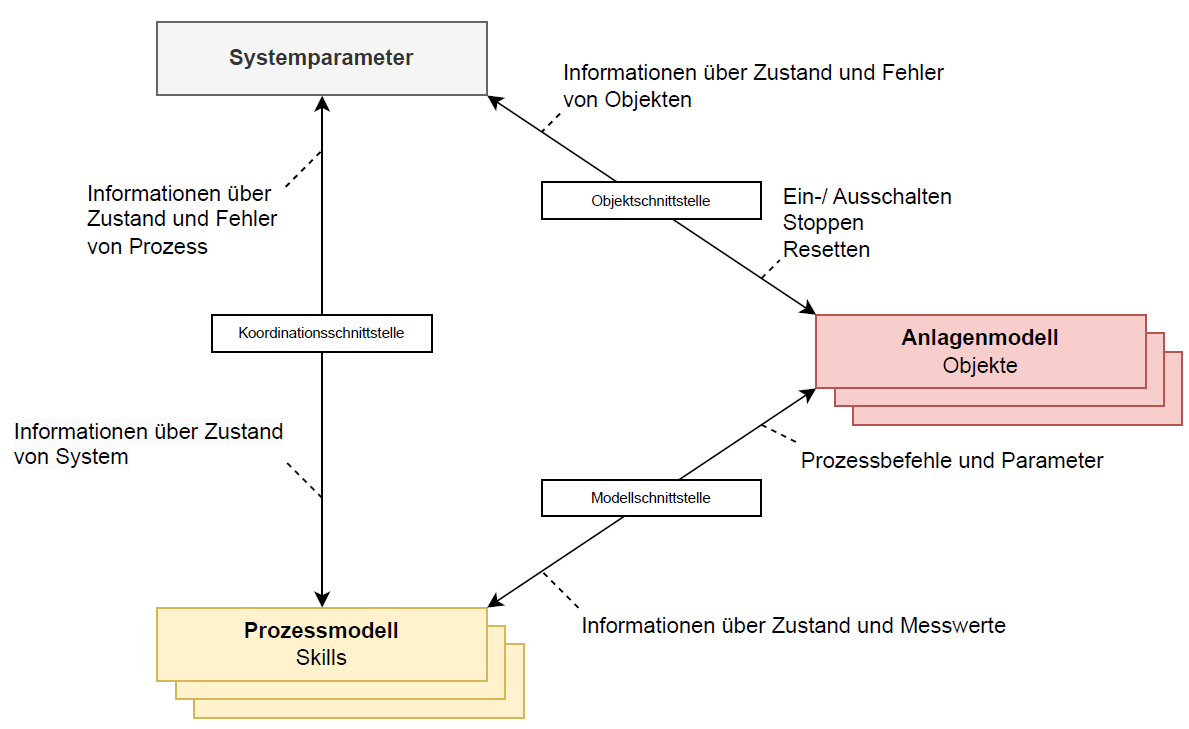
\includegraphics[width=0.6\textwidth]{05_Softwarestruktur/Schnittstellenoverview}
		\captionsetup{justification=centering}
		\caption{Schnittstellenübersicht}
		\label{fig:Schnittstellenübersicht}
	\end{figure}
	
	Die Schnittstellen und deren Abgrenzung dienen als Grundlage für die Bestimmung der Zustände. Dabei werden die Zustände für das System, die Skills und die Objekte bestimmt. Die System- und Objektzustände sind entscheidend für die grundlegende Struktur der Skills, da diese auf die jeweiligen Zustände reagieren müssen. Folglich stellen die definierten System- und Objektzustände lediglich die Mindestanforderungen dar, die notwendig sind, um eine Interaktion mit den Skills zu ermöglichen. Bei der Entwicklung der jeweiligen Systemelemente (Prozessmodell \verb|&| Anlagenmodell) können noch weitere Zustände dazukommen. 
	
	\newpage
	
	\textbf{System:}
	\vspace{2mm} 
	\\
	Das System besitzt mindestens folgende 5 Zustände:
	
	\begin{table}[ht]
		\scriptsize
		\centering
		\colorlet{BFH-table}{BFH-MediumBlue!10}
		\colorlet{BFH-tablehead}{BFH-MediumBlue!50}
		\begin{bfhTabular}{ll}
			Zustand: 		& Beschreibung:															\\\hline
			0 | \verb|AUS| 		& Das System ist ausgeschaltet (Startzustand)							\\\hline
			1 | \verb|BEREIT|	& Das System ist eingeschaltet und bereit einen Prozess durchzuführen	\\\hline
			2 | \verb|LAUFEND| 	& Ein Prozess wird ausgeführt											\\\hline
			3 | \verb|GESTOPPT|	& Ein Prozess wurde gestoppt											\\\hline
			4 | \verb|FEHLER|	& Es gibt einen Fehler im System 
		\end{bfhTabular}
		\captionsetup{justification=centering}
		\caption{Minimale Systemzustände}
		\label{tab:Minimale_Systemzustände}
	\end{table}
	
	\begin{figure}[h!]
		\centering
		\includegraphics[width=0.7\textwidth]{05_Softwarestruktur/Systemzustände}
		\captionsetup{justification=centering}
		\caption{Minimale Systemzustände}
		\label{fig:Minimale_Systemzustände}
	\end{figure}
	
	\textbf{Skill:}
	\vspace{2mm} 
	\\
	Ein Skill besitzt 6 Zustände:
	
	\begin{table}[ht]
		\scriptsize
		\centering
		\colorlet{BFH-table}{BFH-MediumBlue!10}
		\colorlet{BFH-tablehead}{BFH-MediumBlue!50}
		\begin{bfhTabular}{ll}
			Zustand: 			& Beschreibung:															\\\hline
			0 | \verb|BEREIT|		& Der Skill ist bereit einen Prozess auszuführen (Startzustand)			\\\hline
			1 | \verb|LAUFEND| 		& Der Skill führt einen Prozess aus										\\\hline
			2 | \verb|ABGESCHLOSSEN|& Der Prozess wurde abgeschlossen (Durch Objekt)						\\\hline
			3 | \verb|ERREICHT|		& Prozessziel wurde erreicht / Prozess beendet (Durch Skill)   			\\\hline
			4 | \verb|LIMIT|		& Grenzwert wurde überschritten und Prozess wurde abgebrochen 			\\\hline
			5 | \verb|FEHLER|		& Es gibt einen Fehler bezüglich des Prozesses  
		\end{bfhTabular}
		\caption{Minimale Skillzustände}
		\label{tab:Minimale_Skillzustände}
	\end{table}
	
	\begin{figure}[h!]
		\centering
		\includegraphics[width=0.7\textwidth]{05_Softwarestruktur/Skillzustände}
		\captionsetup{justification=centering}
		\caption{Minimale Systemzustände}
		\label{fig:Minimale_Skillzustände}
	\end{figure}
	
	\newpage
	
	\textbf{Objekt:}
	\vspace{2mm} 
	\\
	Ein Objekt benötigt mindestens folgende 7 Zustände:
	
	\begin{table}[ht]
		\scriptsize
		\centering
		\colorlet{BFH-table}{BFH-MediumBlue!10}
		\colorlet{BFH-tablehead}{BFH-MediumBlue!50}
		\begin{bfhTabular}{ll}
			Zustand: 						& Beschreibung:															\\\hline
			0 | \verb|AUS|					& Das Objekt ist ausgeschaltet (Startzustand)							\\\hline
			1 | \verb|BEREIT|				& Das Objekt ist eingeschaltet und bereit								\\\hline
			2 | \verb|LAUFEND| 				& Das Objekt ist aktiv													\\\hline
			3 | \verb|ABGESCHLOSSEN_INTERN|	& Prozess wurde abgeschlossen (Durch Objekt)							\\\hline
			4 | \verb|ABGESCHLOSSEN_EXTERN|	& Prozess wurde abgeschlossen (Durch Skill)								\\\hline
			5 | \verb|GESTOPPT|				& Prozess wurde gestoppt (Durch System)		 							\\\hline
			6 | \verb|FEHLER|				& Es gibt einen Fehler bezüglich des Objektes
		\end{bfhTabular}
		\caption{Minimale Objektzustände}
		\label{tab:Minimale_Objektzustände}
	\end{table}
	
	\begin{figure}[h!]
		\centering
		\includegraphics[width=0.7\textwidth]{05_Softwarestruktur/Objektzustände}
		\captionsetup{justification=centering}
		\caption{Minimale Objektzustände}
		\label{fig:Minimale_Objektzustände}
	\end{figure}
	\vspace{3mm}
	
	Die Definition der allgemeinen Software-Struktur und ihrer Interaktionen bildet die Grundlage für die Ausarbeitung der detaillierten Struktur, Funktionsweise und Implementierung der Skills sowie des Anlagenmodells.
	
	
	